\documentclass[sigconf,nonacm]{acmart}

\settopmatter{printacmref=false,printccs=false,printfolios=true}
\renewcommand\footnotetextcopyrightpermission[1]{}
\pagestyle{plain}
\setlength{\headheight}{16.5pt}

\usepackage{amsmath}
\usepackage{booktabs}
\usepackage{graphicx}
\usepackage{microtype}
\usepackage{multirow}
\usepackage{placeins}
\usepackage{tikz}
\usepackage{pgfplots}
\usepackage{xcolor}
\usepackage{xurl}
\usetikzlibrary{arrows.meta,positioning}
\pgfplotsset{compat=1.18}

\definecolor{adaptivegreen}{HTML}{237A57}
\definecolor{fixedblue}{HTML}{2D6EA3}
\definecolor{orangered}{HTML}{B24A3B}
\definecolor{papergray}{HTML}{60646C}
\definecolor{lightgreen}{HTML}{DDEFE7}
\definecolor{lightblue}{HTML}{DCE9F4}
\definecolor{lightred}{HTML}{F2DDD8}

\graphicspath{{adaptive_npa_figures/}}
\newcommand{\npa}{\mathrm{NPA}}
\newcommand{\anpa}{\mathrm{A\mbox{-}NPA}}

\title{Budgeted Adaptive Neural Particle Automata:
Continuous-Scale Material Resolution Under a Fixed GPU Budget}

\author{Mitchell Mosure}
\email{mitchell@mosure.me}
\affiliation{%
  \institution{Independent Research}
  \city{Chicago}
  \country{USA}
}

\begin{abstract}
Neural Particle Automata (NPA) learn local rules that organize moving
particles into persistent morphologies, but the released formulation assigns
one equal represented measure, interaction scale, and rendered footprint to
every particle. We present a budgeted adaptive NPA substrate that separates
represented material measure, continuous material radius, interaction
bandwidth, execution bins, and Gaussian rendering scale. A conservative paired
topology operation relocates fine resolution while preserving active row
count and total represented material. The implementation is integrated into
the Burn/WGPU NPA runtime, uses device-resident topology and perception, and
trains through a differentiable Target2D rollout with event-aligned truncated
backpropagation through time.

On the released lizard task, one lizard-specific adaptive rule uses 3,070
visible, recurrent, and interacting rows to represent 4,096 fine material
units. Across 32 seeds and four rollout horizons, it obtains 25.31 dB mean
PSNR, including 26.12 dB at 256 steps and 26.32 dB at 512 steps. Its aggregate
gap to the released 4,096-particle oracle is $-0.16$ dB, while interaction work
is 74.95\% and measured wall time is 96.27\% of a same-rule 4,096-row control.
The renderer audit measures 33 occupied material-scale bins and a 2.001$\times$
isotropic Gaussian-radius span with $1.22\times10^{-7}$ relative represented
measure error. These positive averages do not establish production parity:
the 1,024-step mean falls to 24.97 dB, worst per-row oracle gap is
$-3.57$ dB, dynamic allocation improves a static graded cut by only
0.014 dB on average, and broader radius ratios reduce quality. We report these
failure boundaries alongside matched renderer rollouts and a reproducible
claim-to-evidence map.
\end{abstract}

\keywords{neural particle automata, adaptive resolution, smoothed particle
hydrodynamics, Gaussian splatting, morphogenesis, GPU simulation}

\begin{teaserfigure}
  \centering
  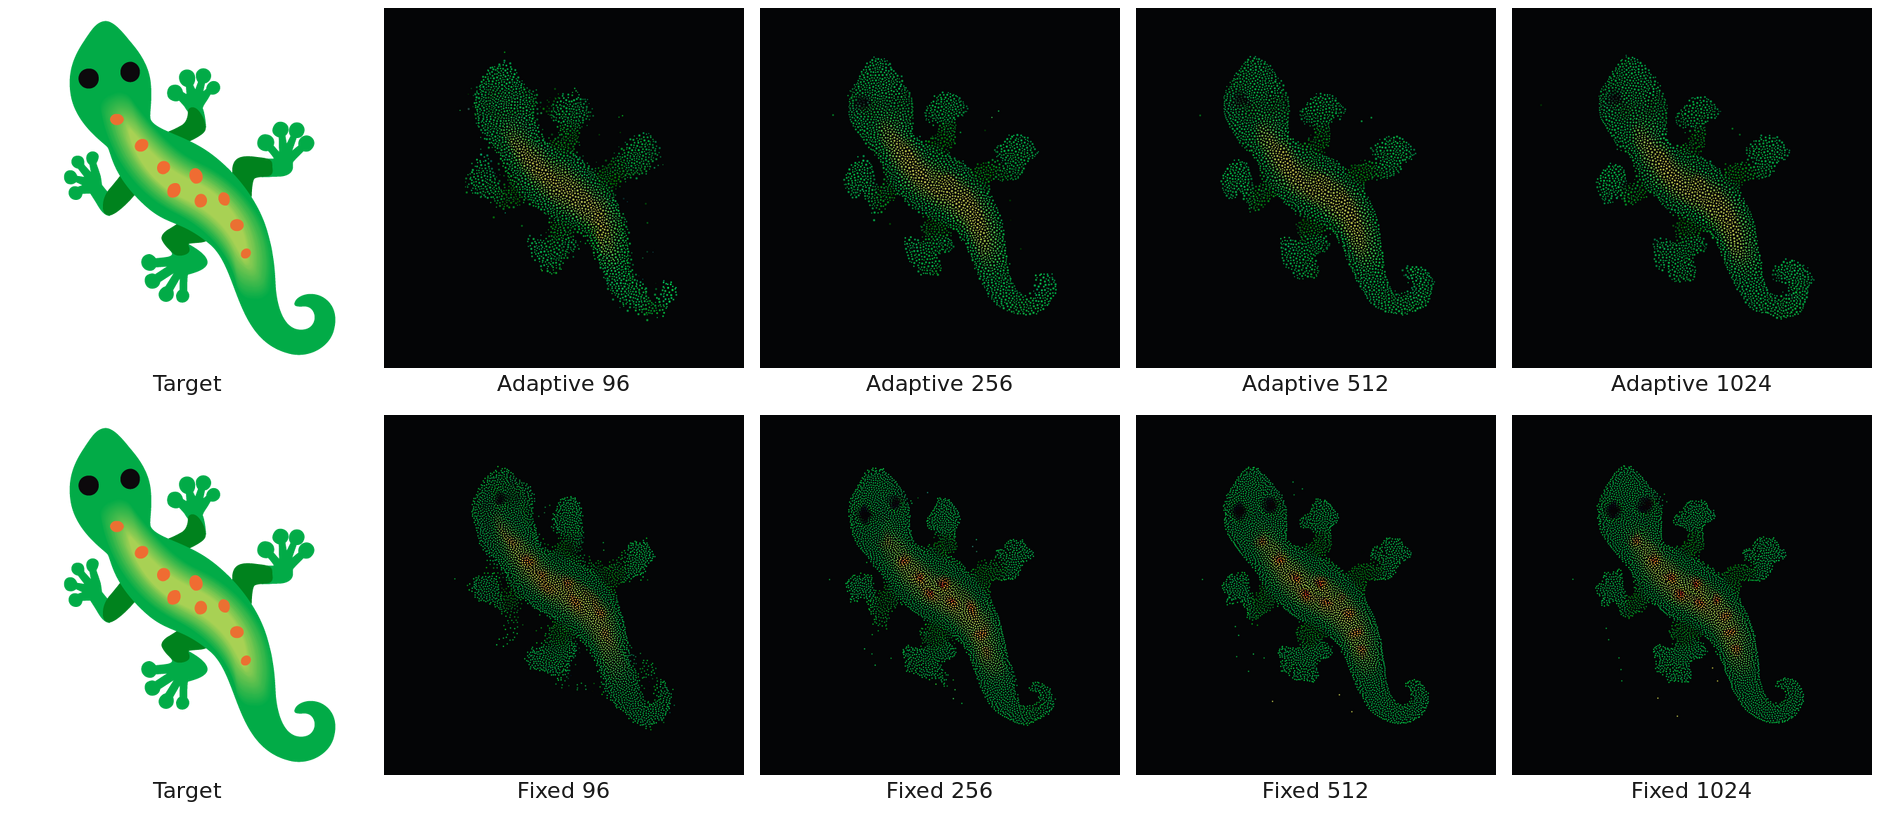
\includegraphics[width=\textwidth]{lizard_rollout_seed42.png}
  \caption{Matched seed-42 Bevy/WGPU rollouts. Top: the adaptive model uses
  3,070 active material rows representing 4,096 fine units. Bottom: the
  released fixed NPA uses 4,096 equal rows. Both are rendered as one isotropic
  Gaussian per active material row at steps 96, 256, 512, and 1,024. The
  adaptive rollout remains recognizable while exposing visibly larger
  coarse-region splats; the fixed oracle retains more fine detail.}
  \Description{A lizard target followed by four adaptive and four fixed NPA
  rollout images at matched time steps.}
  \label{fig:teaser}
\end{teaserfigure}

\begin{document}
\maketitle

\section{Introduction}

Neural cellular automata demonstrate that a compact local rule can grow,
repair, and maintain a global pattern through repeated decentralized
updates~\cite{mordvintsev2020growing}. Neural Particle Automata (NPA) extend
this idea to a Lagrangian substrate: particles carry continuous positions and
latent state, communicate through smoothed particle hydrodynamics (SPH)
operators, and share a small update network~\cite{kim2026npa}. The released
Growing NPA produces detailed two-dimensional morphologies from a seed with
4,096 moving particles.

The fixed discretization is both a strength and a limitation. It gives every
row identical semantic weight, interaction support, and rendered footprint,
which simplifies batching and training. It also spends the same recurrent and
interaction budget in smooth interiors as at thin boundaries, color changes,
and unstable moving fronts. Classical adaptive SPH addresses an analogous
problem through variable smoothing lengths and particle refinement
~\cite{price2012sph,muta2022efficient,nealon2024adaptive}. Applying those ideas
to a learned automaton is not a matter of changing point size. Material
measure, communication reach, topology, recurrent state, and rendering must
remain distinct, and discrete events must not silently duplicate represented
matter or invalidate the learned rule.

This paper replaces an earlier manufactured-oracle design draft with the
measured implementation now present in \texttt{burn\_automata}. We study a
bounded question: can a lizard-specific NPA retain useful quality when 25\%
of its active rows are removed and the remaining rows carry continuous,
conservatively reallocated material scale? We do not claim a learned
scale-free rule, arbitrary particle birth/death, or a generalized 3D adaptive
system.

Our contributions are:
\begin{itemize}
  \item a semantic decomposition of represented measure, material radius,
  interaction bandwidth, execution bins, and Gaussian footprint;
  \item a fixed-budget paired topology operation that relocates fine detail
  without changing row count or total material;
  \item a Burn-native event-aware training and WGPU inference path with
  differentiable recurrent state and device-resident topology; and
  \item a 32-seed, four-horizon evaluation against static, same-rule fine, and
  released-oracle controls, including renderer evidence and negative tails.
\end{itemize}

\section{Related Work}

\paragraph{Neural automata and NPA.}
Growing NCA established differentiable morphogenesis on a regular grid
~\cite{mordvintsev2020growing}. NPA replaces grid convolution with local SPH
perception and allows particles to move~\cite{kim2026npa}. Our recurrent state,
stochastic update mask, growing seed, and two-layer update MLP follow that
work. We change the discretization and renderer contract around the rule.

\paragraph{Adaptive particles.}
Variable-resolution SPH changes particle measure and support while preserving
consistency and conservation~\cite{price2012sph,muta2022efficient}. Corrected
gradients and dual-support interactions matter when support varies
~\cite{bonet1999variational,ren2016dual}; kernel and neighbor choices also
affect stability~\cite{dehnen2012improving}. Our current quality leader keeps
interaction bandwidth fixed, so it is a material-resolution experiment rather
than a complete variable-support solver. The code includes separate bandwidth
and support-bin paths, but the paper does not attribute quality to them.

\paragraph{Gaussian decoding.}
Point-based rendering can attach covariance and opacity to each primitive
~\cite{kerbl2023gaussian}. Our 2D viewer uses the Gaussian-splatting runtime,
but emits one isotropic Gaussian per active material leaf. We derive its radius
from represented measure and do not train arbitrary anisotropic covariance.
This makes the particle budget and the visible primitive budget identical.

\section{Adaptive NPA}

\subsection{Fixed NPA Rule}

Particle $i$ has position $x_i^t\in\mathbb{R}^2$ and latent state
$s_i^t\in\mathbb{R}^{16}$. Compact SPH operators compute smoothed state,
state gradients, and density gradients within support $\epsilon$. A shared
two-layer MLP maps the resulting 66-dimensional perception to position and
state increments. A Bernoulli mask with probability 0.5 applies asynchronous
updates. We use the released normalization and detach positions inside the
perception graph, matching the fixed-rule runtime.

\subsection{Represented Measure and Material Radius}

The adaptive state adds positive represented $q$-measure $\omega_i$ and
separates four notions often conflated as ``scale'':
\begin{equation}
  p_i = (x_i,s_i,\omega_i,\delta_i,h_i,\beta_i,\gamma_i),
\end{equation}
where $\delta_i$ is material radius, $h_i$ is exact interaction bandwidth,
$\beta_i$ is an execution bin, and $\gamma_i$ marks an active material row.
For intrinsic dimension $q$,
\begin{equation}
  \delta_i = \left(\frac{\omega_i}{c_q}\right)^{1/q},
  \qquad c_q=\frac{\pi^{q/2}}{\Gamma(q/2+1)}.
  \label{eq:radius}
\end{equation}
Thus $\delta_i$ is derived state, not a free visual control. The discrete
material measure is
\begin{equation}
  \mu_N = \sum_{i:\gamma_i=1}\omega_i\delta_{x_i}.
\end{equation}
Inactive hierarchy rows and communication proxies are nonmaterial and are not
rendered.

\begin{table}[t]
\caption{Scale semantics. Only represented material determines material
resolution and visible primitive size.}
\label{tab:semantics}
\centering
\small
\begin{tabular}{lll}
\toprule
Quantity & Meaning & Current leader \\
\midrule
$\omega_i$ & represented material & continuous \\
$\delta_i$ & material radius from Eq.~\ref{eq:radius} & continuous \\
$h_i$ & exact interaction support & fixed at 0.1 \\
$\beta_i$ & search acceleration bucket & one occupied \\
$\sigma_i$ & rendered Gaussian radius & $\kappa\delta_i$ \\
$\gamma_i$ & active material ownership & discrete \\
\bottomrule
\end{tabular}
\end{table}

\subsection{Conservative Paired Detail Relocation}

The evaluated model has a fixed resident budget of 3,070 active rows. A local
detail exchange refines one coarse four-unit row into four one-unit rows while
merging four fine rows elsewhere into one coarse row. Each half changes row
count by three in opposite directions, so the complete event preserves the
active count. For a parent $p$ and children $c$,
\begin{align}
  \sum_c \omega_c &= \omega_p,\\
  \sum_c \omega_c x_c &= \omega_p x_p,\\
  \sum_c \omega_c(x_cx_c^\top+\Sigma_c)
    &= \omega_p(x_px_p^\top+\Sigma_p).
  \label{eq:conservation}
\end{align}
Extensive state channels use the same measure weights. Intensive recurrent
state is prolonged locally and recentered. Merge is the inverse weighted
restriction. These equalities protect discrete measure, centroid, and
uncentered second moment; they do not imply that a learned nonlinear rollout
is invariant to resolution.

The controller ranks coarse regions for refinement and fine regions for
coarsening from state and occupancy detail. Accepted exchanges are deterministic
under a fixed seed. The quality experiment schedules eight exchanges every 64
steps between steps 64 and 512. There are no hidden fine rows: visible,
recurrent, and interaction row counts all equal 3,070.

\subsection{Perception and GPU Execution}

SPH sums use represented measure rather than assuming one equal source weight.
The kernel computes measure-weighted density and Shepard-normalized state
features. Burn custom operations expose CubeCL/WGPU/CUDA forward and vector-
Jacobian products for the recurrent perception and Target2D renderer.
Topology ranking and paired exchanges execute on device without copying
particle state to the host. A sorted-cell hash grid bounds candidate search;
the evaluated candidate occupies one support bin because $h_i=0.1$.

Figure~\ref{fig:pipeline} summarizes ownership. The NPA rule predicts motion
and latent state. The topology controller changes where the fixed row budget
is fine. Material measure determines the displayed Gaussian, while the
execution bucket affects only candidate search.

\begin{figure}[t]
\centering
\begin{tikzpicture}[
  node distance=4mm and 4mm,
  box/.style={draw,rounded corners=2pt,minimum height=7mm,align=center,font=\scriptsize},
  arrow/.style={-{Latex[length=2mm]},thick}
]
\node[box,fill=lightblue] (state) {particles\\$x,s,\omega,h$};
\node[box,fill=lightblue,right=of state] (perception) {measure-aware\\SPH perception};
\node[box,fill=lightgreen,right=of perception] (rule) {shared\\NPA rule};
\node[box,fill=lightgreen,below=of perception] (topology) {paired detail\\relocation};
\node[box,fill=lightred,right=of rule] (render) {isotropic\\Gaussian decode};
\draw[arrow] (state) -- (perception);
\draw[arrow] (perception) -- (rule);
\draw[arrow] (rule) -- (render);
\draw[arrow] (rule.south) |- (topology.east);
\draw[arrow] (topology.west) -| (state.south);
\draw[arrow] (rule.north) -- ++(0,3mm) -| (state.north);
\end{tikzpicture}
\caption{Maintained adaptive path. Recurrent dynamics, material allocation,
and rendering have explicit interfaces; Gaussian size is not fed back as an
interaction radius.}
\Description{A block diagram from particle state through SPH perception and
the shared NPA rule to Gaussian rendering, with a paired topology feedback
path.}
\label{fig:pipeline}
\end{figure}

\subsection{Measure-Calibrated Gaussian Rendering}

For the 2D paper captures, each active row emits one isotropic Gaussian:
\begin{equation}
  \Sigma_i^{\mathrm{render}} = \sigma_i^2 I,\qquad
  \sigma_i=\kappa\delta_i.
  \label{eq:gaussian}
\end{equation}
The viewer uses $\kappa=3.84$. Opacity compensates during bounded footprint
transitions so rendered measure cannot be multiplied by showing a parent and
its children simultaneously. The measured axis ratio is exactly one. This
choice is intentionally more constrained than arbitrary-scale anisotropic
Gaussian decoding: the current claim concerns adaptive particle material, not
a separate learned splat representation.

\section{Event-Aware Training}

The adaptive lizard rule starts from a lizard checkpoint trained with scale
conditioning. It is optimized through the alpha-aware Target2D image objective
used by the maintained adaptive trainer. This is not a from-scratch oracle
parity claim. Training uses persistent particle pools and stochastic
asynchronous updates. Truncated backpropagation through time (TBPTT) is aligned
exactly to events. If a topology event lies inside a chunk, the chunk is split at
that step rather than delaying the event. Discrete event selection is detached;
continuous recurrent segments before and after the event remain differentiable.

Gradients from all segments and a bounded post-event recovery window are
accumulated before one Adam update per outer step. An optional paired
degradation term measures the positive increase from a pre-event detached
render to a post-event render; it was rejected because it cost 6--10\%
throughput without improving the broad tail. The quality-scale Target2D
regression keeps recurrent rollout batched, dispatches one device custom
renderer operation per sample row, and concatenates outputs. This avoids a
previous batched-stride corruption while retaining GPU-resident tensors.

Exact-event training sustains 3.05--3.42 million particle-steps/s on an
NVIDIA RTX PRO 6000 Blackwell workstation GPU. The number is a trainer
throughput characterization, not a comparison to the released trainer, whose
hardware and measurement contract differ.

\section{Experimental Protocol}

\subsection{Task and Controls}

We evaluate the released Growing NPA lizard target. Target extraction uses
4,096 points and the numerical image objective renders at $256^2$. The
adaptive candidate uses 3,070 active rows representing 4,096 fine units and a
graded continuous seed with nominal measure ratio four.

Three controls isolate different questions:
\begin{description}
  \item[Static graded.] The same 3,070-row mixed material layout without
  dynamic exchanges tests whether allocation decisions help.
  \item[Same-rule fine.] The adaptive recurrent rule on 4,096 equal fine rows
  tests the cost of removing recurrent degrees of freedom.
  \item[Released oracle.] The published target-specific lizard NPA tests
  external morphology quality under matched seeds and horizons.
\end{description}
The fresh renderer figures compare the adaptive candidate and released oracle.
Numerical PSNR is computed by the differentiable Target2D renderer, not from
the screenshots.

\subsection{Broad Evaluation}

The broad matrix uses seeds 42 through 73 and horizons
$T\in\{96,256,512,1024\}$, yielding 128 seed-horizon rows. All methods use
update probability 0.5, the same uniform-circle seed policy, and uncentered
deployment PSNR. We report aggregate and worst PSNR, oracle and same-rule
gaps, cross-horizon drift, material error, occupancy, overflow, accepted
events, interaction work, and wall time.

Promotion requires more than average parity. The internal quality gate also
checks 1,024-step mean, worst-seed drift, dynamic-over-static gain, and
worst-row oracle gap. This prevents a strong 256--512-step average from hiding
late instability or an inactive allocator.

\section{Results}

\subsection{Morphology Quality}

\begin{table}[t]
\caption{32-seed uncentered deployment PSNR. ``Fine'' uses the same recurrent
rule with 4,096 equal rows; ``oracle'' is the released lizard checkpoint.}
\label{tab:quality}
\centering
\small
\begin{tabular}{rrrrr}
\toprule
Steps & Adaptive mean & Adaptive worst & Fine mean & Oracle mean \\
\midrule
96   & 23.85 & 23.17 & 24.82 & 23.87 \\
256  & 26.12 & 25.14 & 27.15 & 25.57 \\
512  & 26.32 & 25.22 & 27.08 & 26.60 \\
1024 & 24.97 & 23.72 & 25.29 & 25.86 \\
\bottomrule
\end{tabular}
\end{table}

\begin{figure}[t]
\centering
\begin{tikzpicture}
\begin{axis}[
  width=\columnwidth,
  height=5.1cm,
  xlabel={rollout steps},
  ylabel={mean PSNR (dB)},
  xtick={96,256,512,1024},
  ymin=23.3,
  ymax=27.5,
  grid=major,
  legend style={font=\scriptsize,at={(0.5,-0.28)},anchor=north,legend columns=3},
  tick label style={font=\scriptsize},
  label style={font=\small}
]
\addplot[color=adaptivegreen,mark=*,very thick]
  coordinates {(96,23.8527) (256,26.1183) (512,26.3184) (1024,24.9693)};
\addlegendentry{adaptive 3070}
\addplot[color=fixedblue,mark=square*,very thick]
  coordinates {(96,24.8230) (256,27.1480) (512,27.0828) (1024,25.2862)};
\addlegendentry{same-rule 4096}
\addplot[color=orangered,mark=triangle*,very thick]
  coordinates {(96,23.8690) (256,25.5718) (512,26.6034) (1024,25.8614)};
\addlegendentry{released oracle}
\end{axis}
\end{tikzpicture}
\caption{Mean quality peaks at 512 steps. The adaptive candidate exceeds
26 dB at 256 and 512 steps but loses 1.35 dB by step 1,024.}
\Description{A line plot of mean PSNR for adaptive, same-rule fine, and
released-oracle rollouts over four horizons.}
\label{fig:psnr}
\end{figure}

Across all rows, adaptive mean PSNR is 25.31 dB and the mean oracle gap is
$-0.16$ dB. That aggregate alone is misleading. The worst adaptive row is
23.17 dB, the worst oracle gap is $-3.57$ dB, and worst per-seed drift from
peak quality is 2.31 dB. At step 1,024 the adaptive mean is 24.97 dB, below
the 25 dB promotion threshold. Figure~\ref{fig:teaser} shows that the
candidate forms a recognizable lizard, but coarse splats soften thin toes,
spots, and eye boundaries relative to the fixed oracle.

\subsection{Adaptive Behavior}

The broad run accepts 2,048 paired local-detail exchanges with no grid
overflow. Total represented material remains within
$8.31\times10^{-7}$ relative error numerically; the independent renderer audit
measures $1.22\times10^{-7}$. Material radii span 2.001$\times$, occupy 33
audit bins, and 99.8\% of rows fall away from exact endpoint bins. Therefore
the model is not an equal-radius renderer artifact.

Allocation effectiveness is weaker. Dynamic topology improves
scale-to-detail correlation over the static cut by 0.0536 on average, but
improves PSNR by only 0.014 dB; its worst dynamic-minus-static row is
$-0.694$ dB. The implementation demonstrably moves resolution, yet the
learned rule does not consistently convert that movement into image quality.

\begin{figure*}[t]
\centering
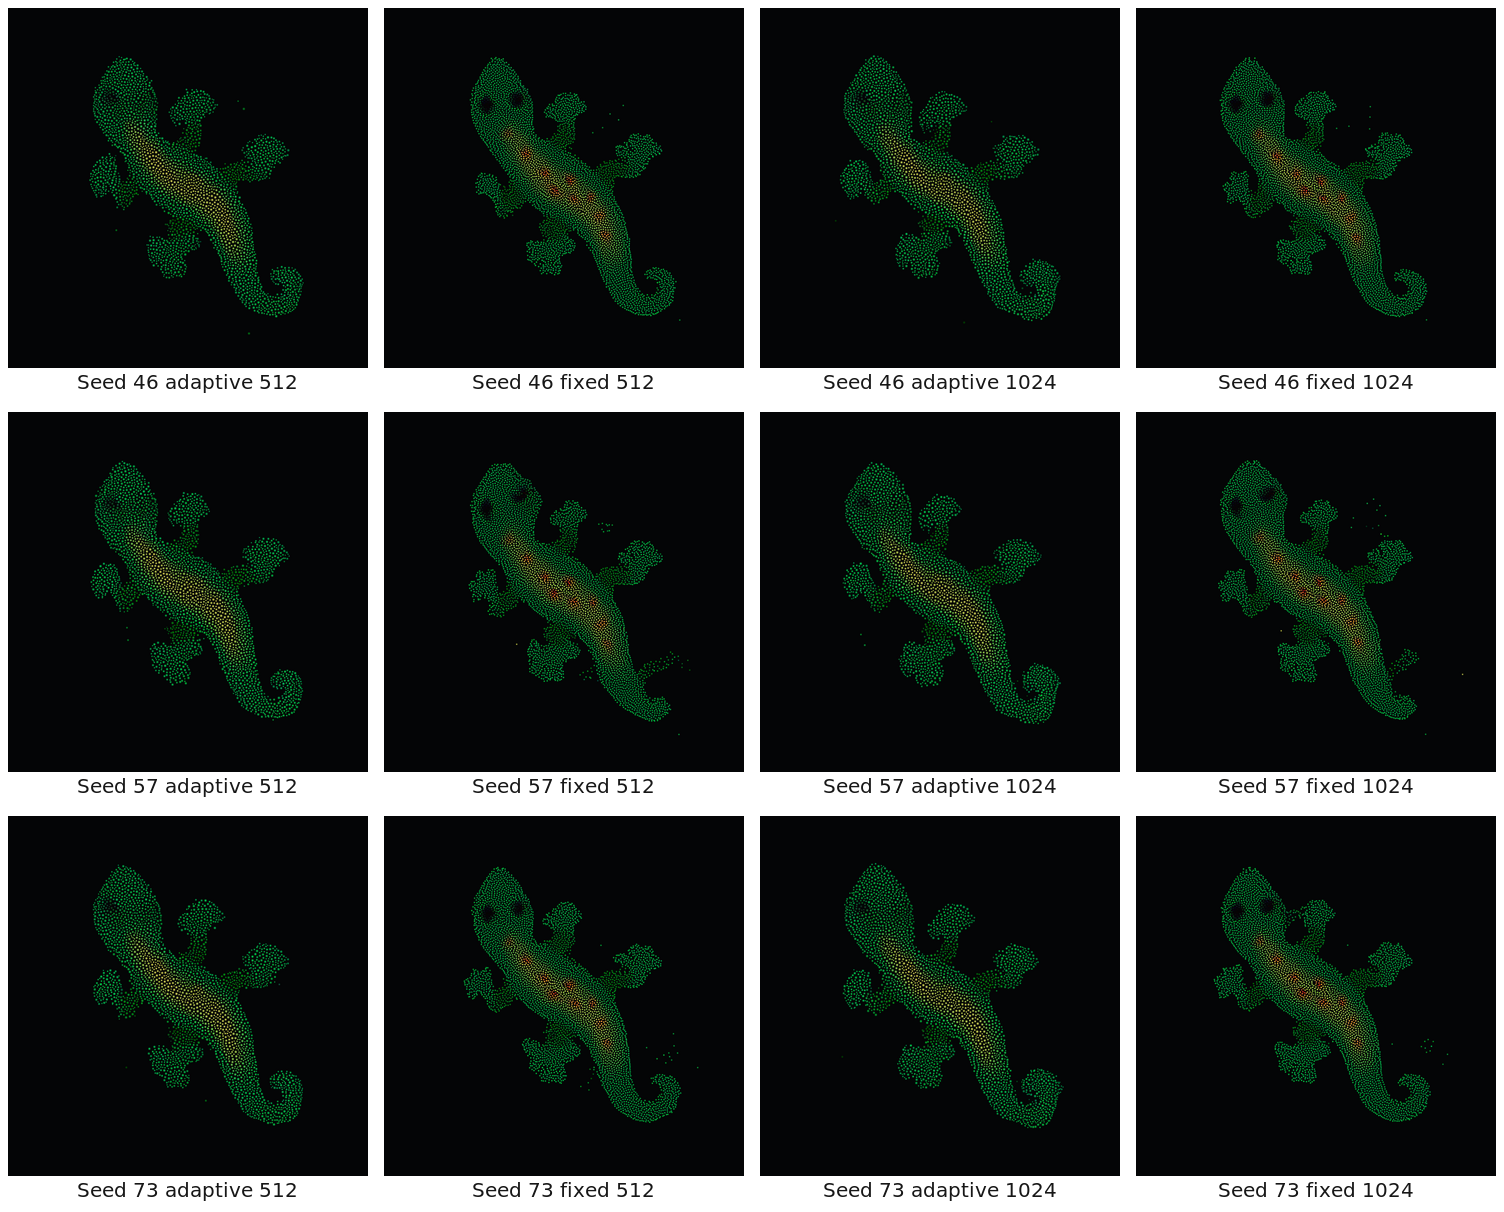
\includegraphics[width=\textwidth]{lizard_seed_robustness.png}
\caption{Matched 512- and 1,024-step rollouts for three seeds. Seed 46 has the
largest measured cross-horizon adaptive drift (2.31 dB); seeds 57 and 73 show
additional stochastic variation. The adaptive rule retains the silhouette,
but the released fixed oracle produces sharper eyes, spots, and extremities.}
\Description{Twelve lizard rollout images arranged by three seeds, adaptive
and fixed models, and two horizons.}
\label{fig:seeds}
\end{figure*}

\subsection{Work and Wall Time}

\begin{table}[t]
\caption{Budget and execution results relative to the same-rule 4,096-row
control. Lower is better for ratios.}
\label{tab:performance}
\centering
\small
\begin{tabular}{lr}
\toprule
Metric & Result \\
\midrule
Active / reference rows & 3,070 / 4,096 \\
Interaction work ratio & 0.7495 \\
Theoretical pair-work ratio & 0.5618 \\
Mean wall-time ratio & 0.9627 \\
Maximum row wall-time ratio & 1.1173 \\
Training throughput & 3.05--3.42 M particle-steps/s \\
\bottomrule
\end{tabular}
\end{table}

The active row reduction translates directly to 74.95\% interaction work.
Quadratic pair-count intuition predicts 56.18\%, but neighborhood construction,
dispatch, topology, and fixed costs prevent that ideal from appearing in wall
time. Mean measured wall time is only 3.73\% lower, and one row is 11.73\%
slower. The result demonstrates bounded GPU execution, not a compelling
end-to-end speedup.

\subsection{Scale and Renderer Audit}

\begin{figure}[t]
\centering
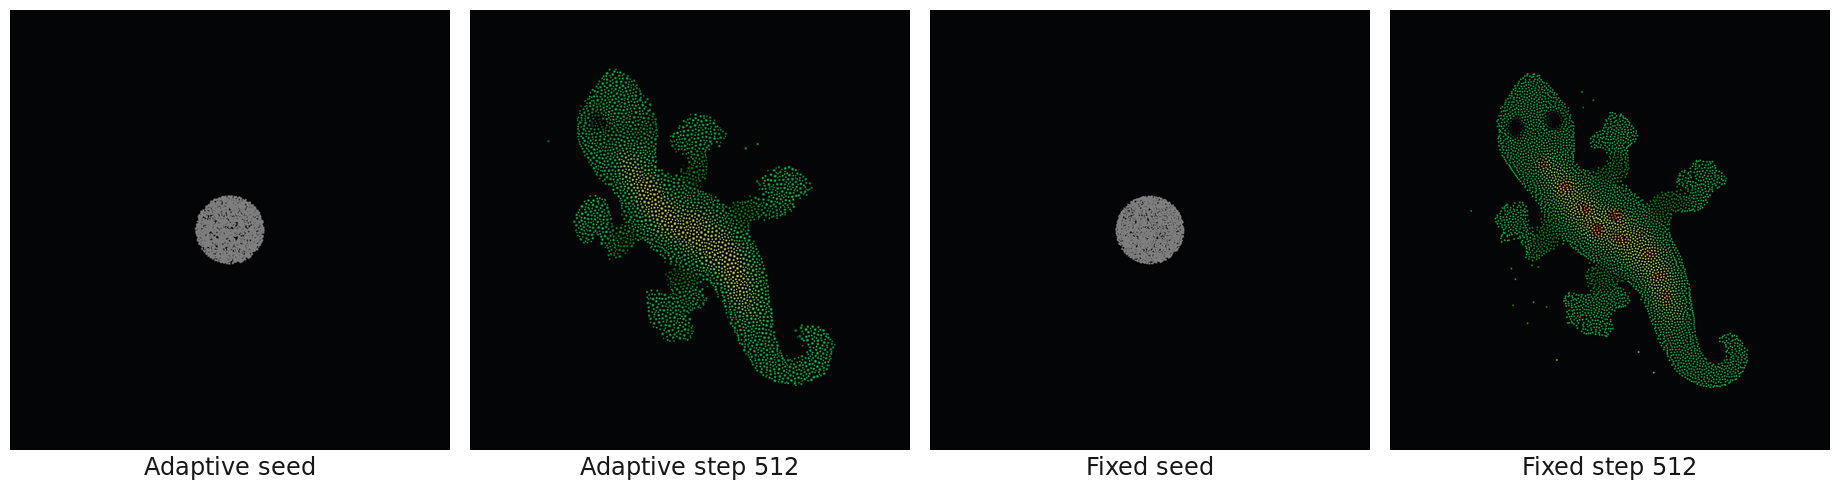
\includegraphics[width=\columnwidth]{lizard_scale_comparison.png}
\caption{Seed and step-512 WGPU captures. The adaptive seed and morphology use
a measured 2.001$\times$ Gaussian-radius span, while the fixed model emits
equal-radius particles. One isotropic Gaussian is drawn per active material
row; parents and active children are never double-rendered.}
\Description{Adaptive and fixed particle seeds and their lizard morphologies
at step 512.}
\label{fig:scale}
\end{figure}

At $768^2$, all audited captures are nonblank. Adaptive Gaussian radius spans
0.009423 to 0.018856 in viewer coordinates, opacity remains within
$[0.9999993,1]$, anisotropic-particle fraction is zero, and maximum axis ratio
is one. Figure~\ref{fig:scale} exposes the intended semantic effect:
coarse material produces a larger primitive from frame zero rather than
growing an arbitrary display radius later in the rollout.

\subsection{Ablations and Failure Cases}

\begin{table}[t]
\caption{Broad or bounded ablations. Drift is worst per-seed loss from peak
PSNR to a later horizon.}
\label{tab:ablations}
\centering
\scriptsize
\begin{tabular}{lrrr}
\toprule
Candidate & Mean & Worst & Drift \\
\midrule
Ratio 4, quality leader & 25.31 & 23.20 & 2.22 \\
Ratio 4, exact-event recovery & 25.35 & 23.18 & 2.47 \\
Ratio 4, paired degradation & 25.34 & 23.19 & 2.73 \\
Ratio 6.25, exact-event & 24.93 & 22.88 & 2.09 \\
Ratio 9, fixed support & 24.65 & 22.63 & 1.97 \\
\bottomrule
\end{tabular}
\end{table}

Exact event alignment slightly raises mean quality but worsens drift.
Explicit post-event degradation training does not repair the tail. Increasing
the measure ratio to 6.25 or 9.0 produces 2.50$\times$ and 3.00$\times$
material-radius spans without touching configured clamps, yet lowers mean and
worst quality. The limitation is learned multiscale dynamics, not a hidden
renderer or feature clamp.

\section{Discussion}

\subsection{What the Experiment Establishes}

The implementation has a real adaptive substrate. Represented measure is
conservative, material and rendered radius vary continuously, topology
relocates detail on device, visible and recurrent budgets match, and 3,070
rows can form a recognizable lizard near the released oracle's average PSNR
over a bounded horizon set. The current result also establishes that an
isotropic measure-calibrated decoder is sufficient to visualize multiscale
particles; arbitrary covariance is not required to observe the adaptive
property.

\subsection{What It Does Not Establish}

This study contains one lizard-specific adaptive rule initialized from a prior
scale-conditioned checkpoint. It does not demonstrate:
\begin{itemize}
  \item from-scratch parity with the official NPA trainer;
  \item a learned rule that generalizes across targets or dimensions;
  \item runtime changes to the total resident row count;
  \item quality-preserving variable interaction bandwidth;
  \item scale-free behavior beyond the measured 2.001$\times$ radius leader;
  \item anisotropic or fully learned Gaussian covariance; or
  \item a robust speedup over the same-rule 4,096-row control.
\end{itemize}
The dynamic allocator's 0.014 dB average gain over a static cut is the most
important negative result. Most quality comes from a competent mixed-scale
rule and seed layout, not from online allocation. Long-horizon event-aware
recovery remains unsolved.

\subsection{Next Experiments}

The next model should optimize a task-risk field that is explicitly predictive
of post-event image loss, rather than using latent-state detail as a proxy.
Training must sample broad seeds and post-event ages, preserve exact event
boundaries, and select checkpoints on worst-seed multi-horizon PSNR and drift.
Only after the ratio-four tail closes should support bandwidth vary; that step
requires dual-support or symmetrized interaction tests and separate backward
parity gates. A variable resident count is a later experiment because it
changes memory ownership and batch shape. Finally, generalized adaptive
HyperNPA requires conditioning both the recurrent rule and allocation policy
across many targets; this paper provides only the substrate and lizard control.

\section{Reproducibility and Claim Boundary}

Source, configuration, reports, and renderer panels are versioned in the
\texttt{burn\_automata} repository~\cite{mosure2026burnautomata}. The bounded
checked-in smoke is:
\begin{verbatim}
configs/verified/adaptive/
  recurrent_target2d_lizard_continuous_
  ratio4_smoke_3070_2d_wgpu.toml
\end{verbatim}
The paper's 32-seed summary is
\path{docs/benchmarks/adaptive_continuous_scale_ratio4_2026-07-25.json};
event-aware ablations are in
\path{docs/benchmarks/adaptive_event_aware_long_horizon_2026-07-25.json}.
The source artifact itself is intentionally gitignored because model weights
are not repository documentation.

The figure manifest records target provenance, export arguments, seeds,
horizons, image dimensions, and SHA-256 hashes. Captures use the release
\texttt{bevy\_automata export} path, 768$\times$768 output, 4,096 requested
particles, update probability 0.5, and matched seeds. The adaptive artifact
emits its stored 3,070 active rows. No paper image is a differentiable-renderer
target or an analytic reconstruction.

\section{Conclusion}

Budgeted adaptive NPA can represent 4,096 fine material units with 3,070
visible and recurrent rows while preserving material, exposing continuous
Gaussian scale, and retaining useful lizard morphology. The measured candidate
exceeds 26 dB mean PSNR at 256 and 512 steps and reduces interaction work by
25.05\%. It does not yet beat fixed NPA as a system: the 1,024-step tail,
weak dynamic-over-static gain, broader-scale regression, and modest wall-time
improvement all fail the stronger promotion standard. Reporting both sides is
essential. The implementation is now a reproducible adaptive substrate and
benchmark, not yet a solved scale-free automaton.

\bibliographystyle{ACM-Reference-Format}
\bibliography{adaptive_npa}

\end{document}
